
%(BEGIN_QUESTION)
% Copyright 2007, Tony R. Kuphaldt, released under the Creative Commons Attribution License (v 1.0)
% This means you may do almost anything with this work of mine, so long as you give me proper credit

This resistor circuit is supposed to function as a precision resistance and voltage divider, for use in a 4-20 mA analog current circuit where one device has a 1-5 volt DC signal input range, and another device has a 0.4-2 volt signal range:

$$\includegraphics[width=15.5cm]{i02277x01.eps}$$

Assume the resistor values shown in the schematic are exact, calculate the required settings for both potentiometers to yield the desired output voltages given a 4 to 20 mA DC input signal range.  Also, determine which of these calibrations should be made first, because one of these potentiometer adjustments affects the other (but not vice-versa)!

\vfil 

\underbar{file i02277}
\eject
%(END_QUESTION)





%(BEGIN_ANSWER)

This is a graded question -- no answers or hints given!

%(END_ANSWER)





%(BEGIN_NOTES)

Given the fact that the entire resistor network should drop 1 to 5 volts over a current range of 4 to 20 mA tells us that it must have a total resistance of 250 ohms.  This allows us to calculate the necessary resistance of the upper potentiometer (connected as a rheostat, or variable resistor).  The only way to get 250 ohms of resistance out of this network is if the right-hand branch (with four resistors) has a resistance of 3375 ohms.  Since the bottom three resistors in this branch have fixed end-to-end resistances, and the only variable resistance is the upper potentiometer, that upper pot must be set for 375 ohms.

\vskip 10pt

Once that has been calculated, we may determine the wiper setting of the lower potentiometer.  If its voltage drop is to be 0.4 volts when the total circuit current is 4 mA (total network voltage drop of 1 volt), we know the voltage divider ratio from the lower pot's wiper to the Gnd terminal must be 40\% of the series resistance in the four-resistor branch.  40\% of the right-hand branch's 3375 ohm total resistance is 1350 ohms.  Subtracting the 1000 ohm value of the lower 1k resistor from this fraction yields 350 ohms from the lower pot's wiper to its bottom terminal.


\vskip 10pt

The upper (1 to 5 volt) pot should be adjusted first, then the 0.4 to 2 volt pot.  This is because the upper potentiometer changes the series resistance in the right-hand branch, thus affecting current through the lower pot, and therefore the influence of the lower pot's wiper setting.  The lower pot, on the other hand, has no effect whatsoever on current in this branch, and therefore has no effect on the setting of the upper pot.

%INDEX% Electronics review: series-parallel resistances

%(END_NOTES)


